\section{Introduction}

The goal of the laboratory was to learn how to use an oscilloscope and a signal generator. We configured the signal, observed various signal shapes and measured signal parameters such as frequency, magnitude, phase shift, period and average value.

\subsection*{Theory}

An oscilloscope, formerly known as an oscillograph, is an instrument that graphically displays electrical signals and shows how those signals change over time.

There are two types of oscilloscopes: analog and digital. An analog oscilloscope captures and displays the voltage waveform in its original form, while a digital oscilloscope uses an analog-to-digital converter to capture and store information digitally. When it comes to debugging and designing, today most engineers use digital oscilloscopes.

\subsection*{A brief history}

The oscilloscope was invented by a French physicist André Blondel in 1893. His device was able to register the values of electrical quantities such as alternative current intensity. An ink pendulum attached to a coil recorded the information on a moving paper tape. The first oscilloscopes had a very small bandwidth, between 10 and 19 kHz.

\subsection*{How does an oscilloscope work?}

To fully understand experiments with an oscilloscope, we have to know how it works.

First of all, an oscilloscope is a combination of various components. But, there are four that are the most important among all. These are:

\begin{itemize}
	\item CRT
	\begin{itemize}
		\item The cathode ray tube is used to display a graph of the voltage or current at a given point in time. The voltage is applied to the cathode, and the ammeter measures the current. The electrons are then accelerated towards the anode, and the voltage controls the beam’s intensity. This creates a beam of electrons that scans the screen from left to right, and the beam’s intensity is proportional to the current.
	\end{itemize}
	\item Vertical control
	\begin{itemize}
		\item Vertical control adjusts the voltage displayed on the screen. The height of the waveforms determines this voltage on the screen. The higher the waveforms, the higher the voltage. The vertical control allows you to adjust the voltage to match the waveforms on the screen.
	\end{itemize}
	\item Horizontal control
	\begin{itemize}
		\item Horizontal control allows the oscilloscope to display a single horizontal line on the screen. It can be used to adjust the timebase, which is the time it takes for the oscilloscope to draw a single horizontal line on the screen. This is measured in milliseconds (ms) and can be adjusted by turning the horizontal control knob.
	\end{itemize}
	\item Triggering control
	\begin{itemize}
		\item Triggering controls the timing of the waveform display. The waveforms are displayed in the time domain, so triggering is used to control the start and stop times of the waveforms. Triggering is also used to control the acquisition of data.
	\end{itemize}
\end{itemize}

\begin{figure}[H]
	\centering
	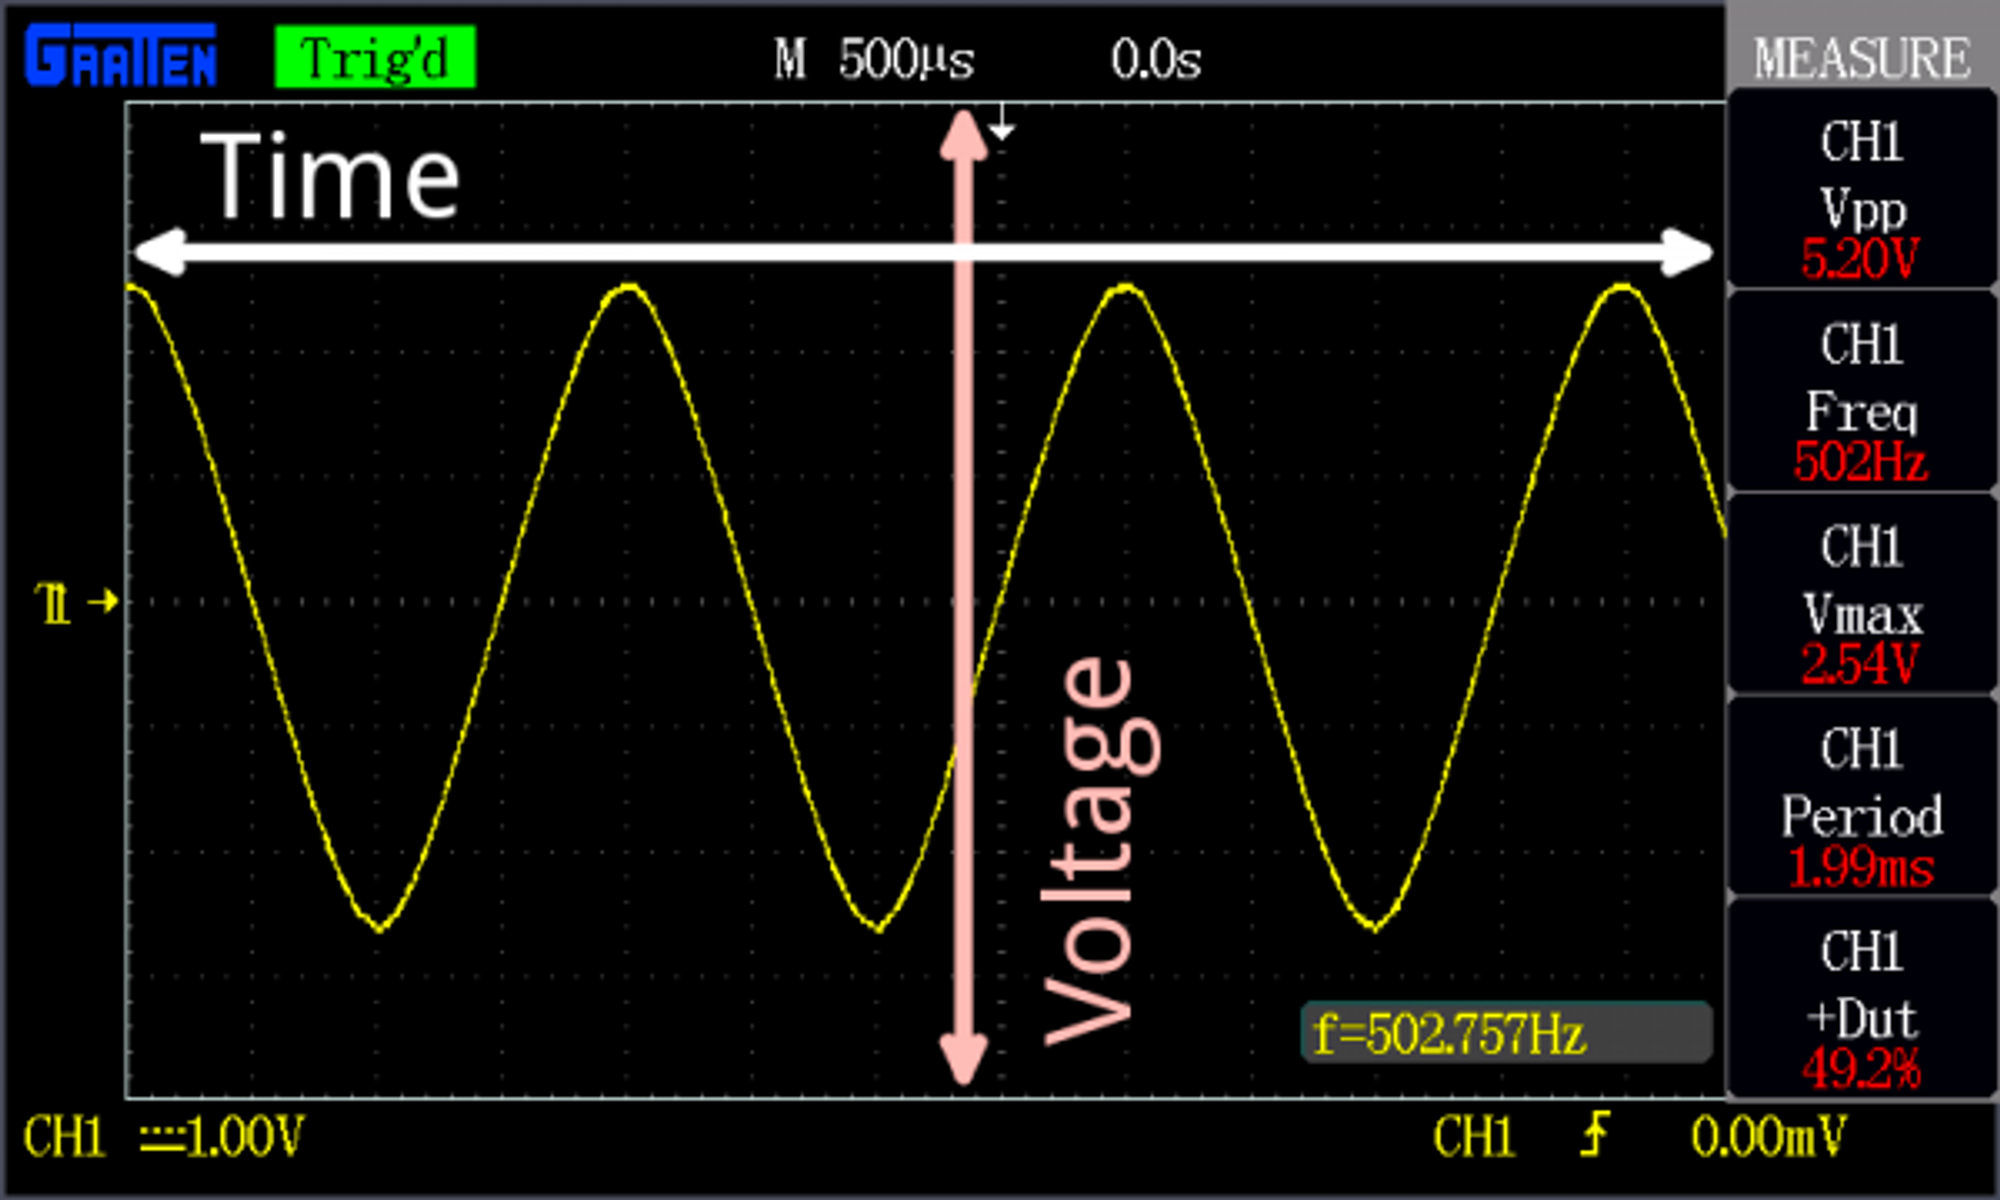
\includegraphics[width=12cm]{images/img.png}
	\caption{Scaled signal in time and amplitude}
	\label{fig:dunno}
\end{figure}

\subsubsection*{Digital Oscilloscope}
A digital oscilloscope can be used to analyze the function of either analog or digital circuits and systems. A typical oscilloscope consists of a cathode ray tube (CRT) with an electron gun, a phosphor-coated screen, and a high voltage power supply. The CRT usually displays time on the x-axis as well as amplitude on the y-axis. Digital oscilloscopes are gaining popularity because they provide more accuracy than their counterparts and many models offer features such as triggering, storage, multiple channels for simultaneous display, math functions such as integration and differentiation, persistence mode for viewing changes in signal over long periods without refreshing the screen every few seconds like most CR.

Digital oscilloscopes work by sampling voltage at a fixed rate and displaying the voltage waveforms on a digital screen. The voltage waveforms are displayed as a series of dots representing the voltage amplitude at a specific point in time. The oscilloscope samples the voltage waveforms at a fixed rate and calculates the average voltage between the samples. This process is repeated for every sample, and the resulting waveform is displayed on the oscilloscope’s screen.

\begin{figure}[H]
	\centering
	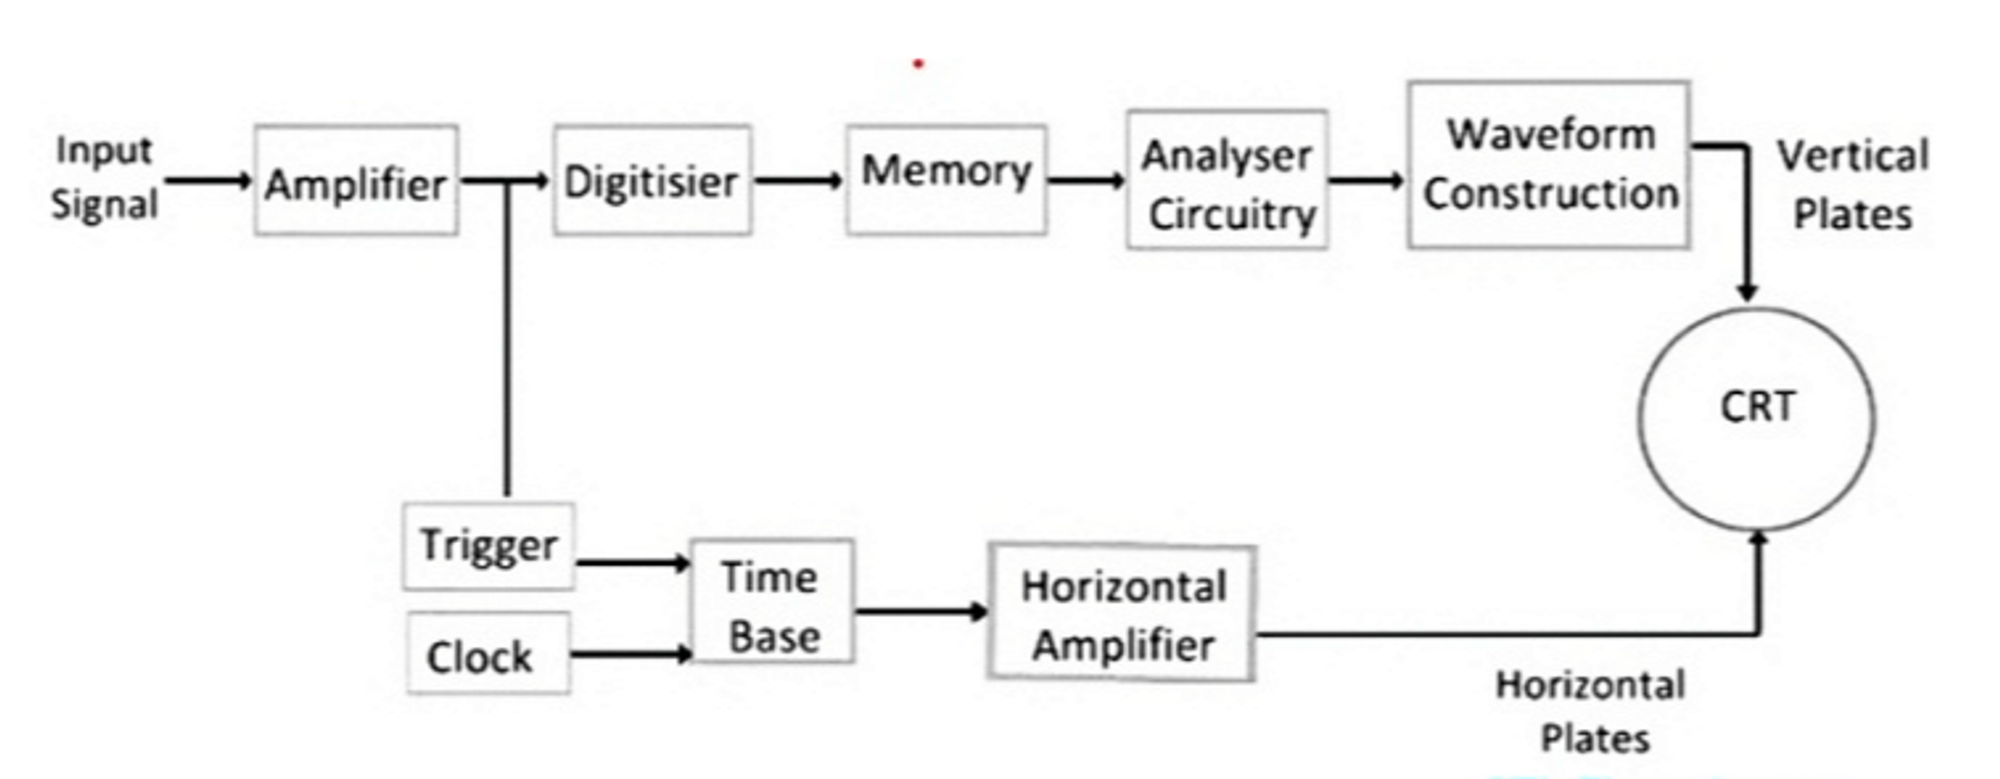
\includegraphics[width=12cm]{images/img_1.png}
	\caption{Schematic example}
	\label{fig:dunno-vol-2}
\end{figure}


















